\chapter{Stand der Wissenschaft}
\label{ch:standderwissenschaft} 


%
% Section: FZ 1.1. Aufbau und Struktur medizinischer Texte 
%
\section{FZ 1.1. Aufbau und Struktur medizinischer Texte}
\label{sec:fz1.1.} 

Medizinische Texte existieren in verschiedenen Formen mit unterschiedlichen Zielsetzungen. Beispielsweise gibt es Lehrbuch- und Enzyklopädietexte, die überblicksweise über medizinische Sachverhalte informieren, wissenschaftliche Studien, in denen neue wissenschaftliche Erkenntnisse vorgestellt werden und außerdem Arztberichte, in denen über individuelle Patienten und deren Krankheitsverlauf informiert wird.
Die für diese Arbeit genutzten Analysetexte stellen enzyklopädische Texte dar, in denen insbesondere Symptome und Merkmale psychologischer Erkrankungen beschrieben werden.
Charakterisiert sind diese Texte dadurch, dass sie durch Zwischenüberschriften gegliedert sind und neben Fließtext auch Aufzählungen enthalten.


%
% Section: FZ 2.1. Überblick über depressive Erkrankungen 
%
\section{FZ 2.1. Überblick über depressive Erkrankungen}
\label{sec:fz2.1.} 
Als Quellen für diesen Abschnitt dienten \cite{mpg_depression}, \cite{who_depression} und \cite{psychrembel_depression}.
\subsection{Allgemein}
Depression ist eine psychische Krankheit, die geschätzt $3,8 \%$ der Weltbevölkerung und $5\%$ der Erwachsenen betrifft.
Sie kann dazu führen, dass betroffene Menschen Schwierigkeiten haben im Arbeits- und Familienleben zurecht zu
kommen, und sie führt im schlimmsten Fall zur Selbsttötung.

\subsection{Symptome}
Übliche Symptome eine Depression sind eine traurige Grundstimmung, Konzentrationsprobleme, Hoffnungslosigkeit, 
Müdigkeit und Reizbarkeit. Auch Schlafstörungen, eine Libidostörung, verminderter oder gesteigerter Appetit und
ein vermindertes Selbswertgefühl oder Selbstbewusstsein sind Symptome. Im schlimmsten Fall treten 
Selbsttötungsgedanken auf.

\subsection{Formen der Depression}
Die Schwere einer typischen Depression wird durch leichte, mittelgradige und schwere Episoden unterschieden. Dabei 
sind die Übergänge fließend.
Besondere Formen der Depression sind die chronische Depression, bei der trotz therapeutischer Maßnahmen nur wenig 
Besserung eintritt. Desweiteren gibt es die manisch-depressive Depression, bei der sich depressive und manische 
Phasen abwechseln. Außerdem gibt es auch kurze, akute depressive Verstimmungen, die nur zwischen einem Tag und
zwei Wochen dauern. 

\subsection{Ursachen}
Depressionen entstehen durch ein kompexes Zusammenspiel von sozialen, psychologischen und biologischen Faktoren.
Dabei wird angenommen, dass für eine typische Depression die Genetik 50% der Ursachen ausmacht. 
Konkret können Kindheitserfahrungen, Verluste und Arbeitslosigkeit eine Depression begünstigen.

\subsection{Behandlung}
Je nach Schweregrad der Krankheit werden zur Behandlung von Depressionen psychologische Behandlungen angewandt, 
und/oder den betroffenen Personen Antidepressiva verschrieben.


%
% Section: FZ 2.2. Automatisierung durch NLP 
%
\section{FZ 2.2. Automatisierung durch NLP}
\label{sec:fz2.2.} 

\subsection{Natural Language Processing (NLP)}
Natural Language Processing ist ein Teil der Künstlichen Intelligenz. Er befasst sich mit der Aufgabe
Maschinen den Umgang mit der menschlichen Sprache beizubringen, also das Verstehen der Sprache und dem
richtigen Antworten darauf. Mithilfe von NLP-Methoden werden zum Beispiel Sätze analysiert, die Bedeutung 
von Texten erfasst, Chatbots erstellt und sogar ganze Geschichten geschrieben.
Die grundlegendsten Schritte, die beim Erarbeiten eines NLP-Modells (oder allgemeiner eines 
Machine-Learning-Modells) ausgeführt werden, sind folgende:
\begin{enumerate}
	\item Aufbereitung von Daten
	\item Wählen eines geeigneten Algorithmus
	\item Trainieren des Modells mit Trainingsdaten
	\item Testen des Modells mit Testdaten
	\item Modell anwenden / Vorhersagen treffen
\end{enumerate}

\subsection{Named Entity Recognition (NER)}
Named Entity Recognition bezeichnet einen Teilbereich des Natural Language Processing, bei dem es darum geht 
wichtige Entitäten, wie zum Beispiel Personen, Orte oder Institutionen, in einem Text zu erkennen. Methoden 
zur Bewältigung dieser Aufgabe werden seit circa 30 Jahren entwickelt. Darunter fallen grammatikbasierte und 
statistische Methoden, sowie auch Methoden des Machine Learning.

\subsection{Entity Linking}
Als Entity Linking wird im Bereich des NLP die Aufgabe beschrieben, die den Entitäten (z.B. Personen, Orte) 
in einem Text das korrekte Äquivalent in einer Wissensbasis zuordnen soll.
In \cite{shen_entity_2021} wird Entity Linking folgendermaßen definiert (übersetzt):
\begin{defn}[Entity Linking]
Gegeben sei ein Dokument $D$, welches die erkannten Entitäten $M=\{m_1, m_2, \dots, m_{|M|}\}$ enthält, sowie
eine Ziel-Wissensbasis $KB$, welches die Entitäten $E=\{e_1, e_2, \dots, e_{|M|}\}$ enthält. Das Ziel ist es 
jede Entität $m_i$ in $M$ seinem korrekten Äquivalent $e_i$ in $E$ zuzuordnen.
\end{defn}

\subsection{spaCy}
spaCy ist eine Python-Bibliothek, die die erforderlichen Daten und Algorithmen enthält, die zum verarbeiten von
Texten mit natürlicher Sprache benötigt werden. SpaCy enthält vortrainierte Modelle für über 70 verschiedene 
Sprachen, unter anderem Spanisch, Englisch, Griechisch und Deutsch. Zudem ermöglicht spaCy das Einbinden von 
Modellen, die mithilfe anderer Python-Bibliotheken (zum Beispiel PyTorch oder TensorFlow) trainiert wurden.
Anders als einige andere NLP-Bibliotheken konzentriert sich spaCy darauf, Software für den Produktionseinsatz 
zur Verfügung zu stellen. Erstmals wurde spaCy 2015 von Matthew Honnibal veröffentlicht. 
\cite{vasiliev2020natural} \cite{github_spacy} \cite{spacy}

\subsection{Weitere Python-Bibliotheken für Machine Learning (ML) und NER}
Eine der wichtigsten Python-Bibliotheken für NLP ist NLTK (Natural Language Toolkit) \cite{bird2006nltk}.
Weitere Python-Bibliotheken, die für NLP-Aufgaben genutzt werden können, sind unter Anderem
Gensim \cite{vrehuuvrek2011gensim}, Pattern \cite{de2012pattern}\cite{github_pattern}, 
scikit-learn und PyTorch.

%
% Section: FZ 1.1. Wissensrepräsentation mittels RDF
%
\section{FZ 3.1. Wissensrepräsentation mittels RDF}
\label{sec:fz3.1.} 

Das \emph{Resource Description Framework} (RDF) \citep{w3c_all_2022} ist ein Framework zur Darstellung von Informationen im Semantischen Web, das von der \emph{RDF Working Group} des  \emph{World Wide Web Consortium} (W3C) erstellt wurde. Das RDF-Modell besteht aus einem Datenmodell, mit dem Aussagen über Ressourcen in Form eines Graphen dargestellt werden. Die Informationen werden als Tripel von Subjekt, Prädikat und Objekt gespeichert und ermöglichen auf diese Weise eine maschinenlesbare Bereitstellung semantischer Informationen.

Die Subjekte und Objekte sind dabei die Knoten des Graphen und die Prädikate die Kanten zwischen diesen Knoten.

Abbildung \ref{fig:rdfgraph} zeigt einen einfachen RDF-Graphen, in dem das Subjekt \glqq depression\grqq{} mit dem Prädikat \glqq hasSymptom\grqq{} mit zwei Symptomen verbunden und über das Prädikat \glqq isA\grqq{} mit dem Objekt \glqq mentalDisorder\grqq{} verbunden ist.

\begin{figure}[h]
    \centering
    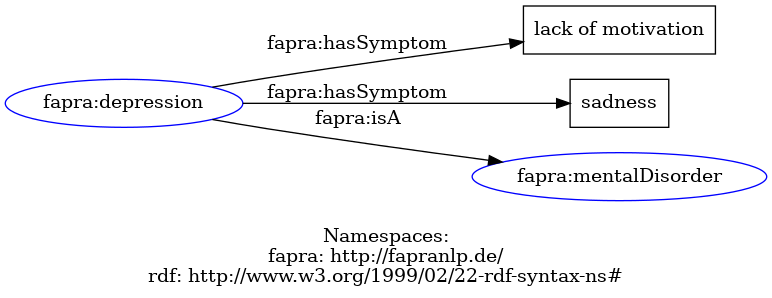
\includegraphics[width=\textwidth]{pictures/rdf-graph.png}
    \caption{einfacher RDF-Graph (visualisiert mit \url{https://www.ldf.fi/service/rdf-grapher}}
    \label{fig:rdfgraph}
\end{figure}

\subsection{Resource Description Framework Schema}

Zusätzlich zu RDF stellt das W3C auch eine Empfehlung für ein Datenmodellierungsvokabular für RDF-Daten bereit: das RDF-Schema. Dies stellt eine Erweiterung des grundlegenden RDF-Vokabulars dar. \dots{} [TODO]

\subsection{Dublin Core Metadata Initiative}
DCMI \dots{} [TODO]

\subsection{Serialisierung von RDF-Graphen}

Für die Serialisierung von RDF-Graphen stehen mehrere Formate zur Verfügung. So wird der MeSH-Datensatz im \emph{N-Triples}-Format bereitgestellt und in diesem Praktikum erfolgt die Ausgabe der Wissensrepräsentation im RDF/XML-Format.

Ein Beispiel für die Serialisierung des in Abbildung \ref{fig:rdfgraph} dargestellten Graphen im RDF/XML-Format ist in Listing \ref{listing:rdfxml} angeführt.

\lstset{language=XML, caption=RDF/XML, label=listing:rdfxml}
\begin{lstlisting}
<?xml version="1.0" encoding="utf-8"?>
<rdf:RDF
  xmlns:fapra="http://fapranlp.de/"
  xmlns:rdf="http://www.w3.org/1999/02/22-rdf-syntax-ns#"
>
  <rdf:Description rdf:about="http://fapranlp.de/depression">
    <fapra:hasSymptom>lack of motivation</fapra:hasSymptom>
    <fapra:hasSymptom>sadness</fapra:hasSymptom>
    <fapra:isA rdf:resource="http://fapranlp.de/mentalDisorder"/>
  </rdf:Description>
</rdf:RDF>
\end{lstlisting}




Für Python steht mit RDFLib \cite{rdflib_team_rdflib_2022} eine Bibliothek zur Arbeit mit RDF-Graphen bereit.

\subsection{SPARQL Protocol and RDF Query Language}
SPARQL \dots{} [TODO]